\documentclass[a4paper,10pt]{article}

\usepackage[utf8]{inputenc}
\usepackage{graphicx}
\usepackage{fancybox}
\usepackage{verbatim}
\newcommand{\HRule}{\rule{\linewidth}{0.5mm}}

\begin{document}

\begin{titlepage}

\begin{center}


% Upper part of the page


\textsc{\LARGE Simulación de Sistemas 72.25}\\[1.5cm]

\textsc{\Large Simulación de un Centro de Mantenimiento para Unidades de Transporte de Pasajeros}\\[0.5cm]


% Title
\HRule \\[0.4cm]
{ \huge \bfseries Trabajo Práctico Final}\\[0.4cm]

\HRule \\[1.5cm]

% Author and supervisor
\begin{minipage}{0.4\textwidth}
\begin{flushleft} \large
\emph{Authors:}\\
Alberto Miguel \textsc{Pose}\\
Juan Ignacio \textsc{Catalano}\\
Martín \textsc{Palombo}\\
Santiago José \textsc{Vazquez}\\
\end{flushleft}
\end{minipage}

\vfill

\end{center}
\thispagestyle{empty}
\end{titlepage}


\section{Punto (a)}
Se modelaron los intervalos de tiempos entre arribos y el tiempo de servicio de ER a partir de los datos provistos en los archivos históricos \verb|arriboscop| y \verb|ercop| respectivamente. Para ello, se graficaron los histogramas correspondientes. En la Figura \ref{fig:hist_arriboscop} vemos el histograma correspondiente a los intervalos de tiempos entre arribos. Para la elección de los intervalos de clase se utilizó el criterio de Nuñez. Como podemos ver intuitivamente, la distribución de los datos en este caso es una triangular. En la Figura \ref{fig:hist_servicios} podemos ver el histograma correspondiente a los tiempos de servicios de ER. De nuevo, intuitivamente podemos ver que la distribución en este caso es una exponencial. Para verificar nuestras hipótesis ejecutamos el test $\chi^2$ sobre dichos datos y pudimos confirmar ambas distribuciones.

\begin{figure}[h]
\begin{center}
\includegraphics[width=15cm]{../src/parteA/hist_arribos.eps}
\caption{\label{fig:hist_arriboscop} Histograma correspondiente a los intervalos de tiempos entre arribos.}
\end{center}
\end{figure}

\begin{figure}[h]
\begin{center}
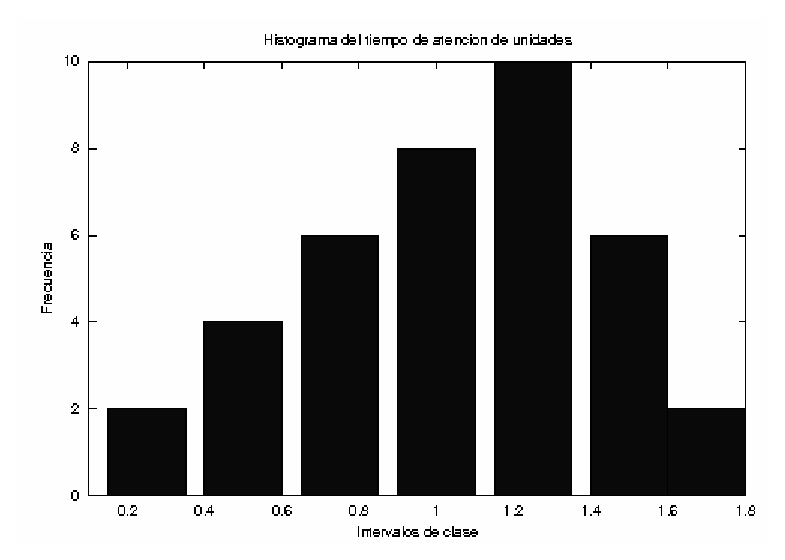
\includegraphics[width=15cm]{../src/parteA/hist_servicios.eps}
\caption{\label{fig:hist_servicios} Histograma correspondiente a los tiempos de servicios de ER.}
\end{center}
\end{figure}

\section{Punto (b)}
Las colas del sistema se denominan como se muestra en la Figura \ref{fig:events_diagram}. Como podemos ver, quedan
determinadas por el conjunto 
\[
S = \{UI, ER1, ER2, ER3, ST\}
\]
El estado del sistema se encuentra compuesto por la longitud y el estado de servicio (busy/free) de cada una de las 3 colas. Las características del sistema, determinan que todas las colas se modelan como de capacidad infinita y utilizan la disciplina FIFO (First In First Out).

\section{Punto (c)}
Los eventos de nuestro sistema quedan definidos por las llegadas y partidas de una UI a cada una de las etapas del proceso de mantenimiento. Como podemos ver en la Figura \ref{fig:events_diagram}, los tipos de eventos estan dados por el conjunto
\[
 E = \{IUI, OUI, IER, OER, IST, OST\}
\]
Como asumimos que la salida de una sección y paso a la próxima se realiza instantaneamente, podemos unificar los tipos de eventos $OUI$ con $IER$ y $OER$ con $IST$. Por lo tanto $E$ nos queda reducido a
\[
 E = \{IUI, IER, IST, OST\}
\]

\begin{figure}[h]
\begin{center}
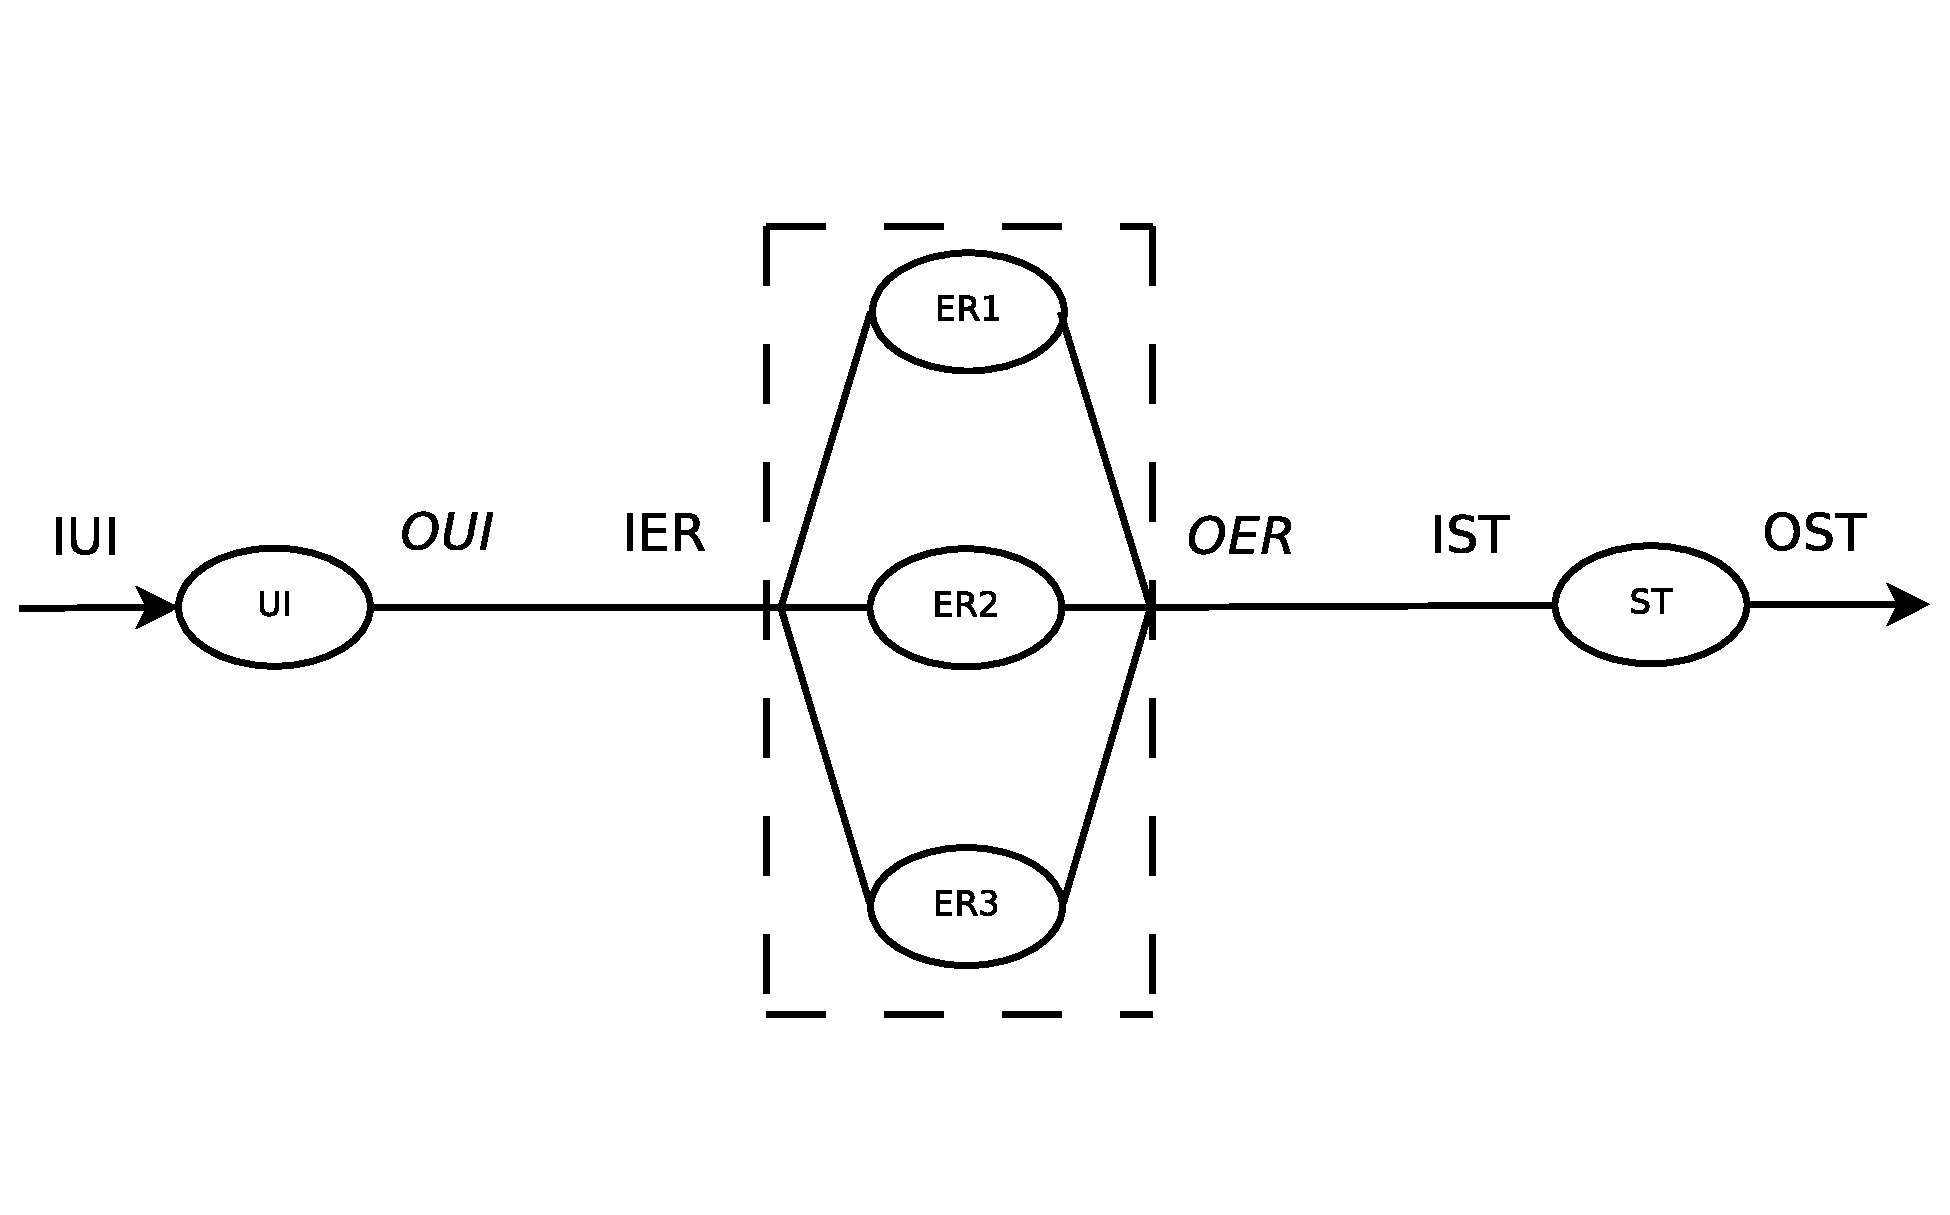
\includegraphics[width=12cm]{./states.eps}
\caption{\label{fig:events_diagram} Diagrama de estados del sistema.}
\end{center}
\end{figure}

\section{Punto (d)}

\section{Punto (e)}

\section{Punto (f)}

\end{document}